\documentclass[a4paper,11pt]{article}

\usepackage[activate={true,nocompatibility}]{microtype}
\usepackage[T1]{fontenc}
\usepackage{microtype}
%\usepackage{mlmodern}
%\usepackage{Baskervaldx}
\usepackage[xcharter]{newtx}

\renewcommand{\baselinestretch}{1.05}
%\usepackage{MnSymbol}
\usepackage{inconsolata}
\usepackage[scaled=0.92]{sourcesanspro}
\usepackage{xcolor}
\usepackage[utf8]{inputenc}
\usepackage[english]{babel}
\usepackage[a4paper, left=1.3in, right=1.3in]{geometry}
\usepackage{calc}
\usepackage{graphicx}

\usepackage{titlesec}

\titleformat{\subsubsection}[runin]
  {\normalfont\itshape}
  {\normalfont\bfseries(\thesubsubsection)}
  {1.5\wordsep}
  {}
  [.]

\titlespacing*{\subsubsection}
  {0pt}{6pt}{\wordsep}  % left, before, after spacing

\usepackage{mathpartir}
\usepackage{amsmath}

\usepackage{listings}
\lstdefinestyle{wasm}{
  basicstyle=\ttfamily,
  numberstyle=\footnotesize,
  numbers=left,
  columns=fullflexible,
  numbersep=10pt,
}
\lstset{style=wasm}

\DeclareMathOperator{\reft}{\textsf{ref}}
\DeclareMathOperator{\rect}{\textsf{rec}}
\DeclareMathOperator{\parat}{\textsf{param}}
\DeclareMathOperator{\rest}{\textsf{result}}
\DeclareMathOperator{\strt}{\textsf{struct}}
\DeclareMathOperator{\arrt}{\textsf{array}}
\DeclareMathOperator{\funt}{\textsf{func}}
\DeclareMathOperator{\fldt}{\textsf{field}}
\DeclareMathOperator{\vart}{\textsf{var}}
\DeclareMathOperator{\cstt}{\textsf{const}}
\DeclareMathOperator{\broncast}{\textsf{br\_on\_cast}}
\DeclareMathOperator{\reftest}{\textsf{ref.test}}
\DeclareMathOperator{\localget}{\textsf{local.get}}
\DeclareMathOperator{\refnullt}{\textsf{ref null}}

\usepackage{tikz}
\usepackage{wrapfig}

\usepackage[backend=bibtex, style=alphabetic]{biblatex}
\addbibresource{report/report.bib}
\renewcommand*{\bibfont}{\small}

\author{Aghilas Y. Boussaa \texttt{<aghilas.boussaa@ens.fr>}}

\title{\textsf{watib}: An optimising toolchain for modern WebAssembly}
\begin{document}
\sloppy
\maketitle
\begin{abstract}
  WebAssembly (Wasm) is a code format providing efficient and safe execution.
  The latest drafts of its standard offer features making it a suitable
  compilation target for functional programming languages. These features led to
  the development of Wasm backends for compilers such as the Bigloo Scheme
  compiler. However, Bigloo's Wasm backend relied on binaryen, an external
  toolchain with user-friendliness and spec-compliance issues.

  We present \textsf{watib}, a new WebAssembly Toolchain written In Bigloo. This
  toolchain is integrated into the Bigloo compiler and is also available as a
  standalone tool. We compare \textsf{watib} with binaryen, showing how the
  former deals with the mentioned issues of the latter. We also benchmark
  \textsf{watib}'s optimisation passes.
\end{abstract}

\section{Introduction}
In 2024, a Wasm backend was added to the Bigloo Scheme compiler~\cite{Bigloo}.
This backend produced textual Wasm and relied on an external toolchain to
assembly it into the binary format. We developed \textsf{watib} as a replacement
for this toolchain. It is part of the Bigloo compiler and is also available as a
standalone tool with a command-line
interface\footnote{\url{https://www.normalesup.org/~boussaa/watib/}}.

The rest of this section gives an overview of WebAssembly and \textsf{watib}.
Section~\ref{val} details \textsf{watib}'s type checker. Section~\ref{opt}
describes the different optimisation passes. Section~\ref{bench} compares
\textsf{watib}'s and existing tools' performances, and Section~\ref{sbbv}
discusses a work-in-progress optimisation. This presentation omits the assembly
phase as, once we have an intermediate representation, it is a straightforward
transcription of the specification.
\subsection{WebAssembly}
WebAssembly~\cite{haas2017bringing} is an assembly-like language for a
stack-based virtual machine. It aims at providing a fast, safe and portable
language endowed with an efficient binary format. Unlike traditional assembly,
Wasm is statically typed and only supports structured control flow. Support for
Wasm in existing compilers is growing~\cite{emscripten, kotlin, ocaml}.

\subsubsection{The standard}
The WebAssembly specification~\cite{WebAssemblyCoreSpecification3} specifies
typing rules (called validation rules), operational semantics, an abstract
representation of Wasm modules, on which the previous rules are stated, and two
grammars for concrete formats. The binary format represents WebAssembly modules
as a sequence of bytes. Wasm virtual machines such as V8~\cite{V8} or
SpiderMonkey~\cite{SpiderMonkey} and toolchains such as binaryen~\cite{Binaryen}
or wasm-tools~\cite{WasmTools} receive this format. The textual format
represents WebAssembly modules as S-expressions. Toolchains receive this format
and humans (and compilers such as Bigloo) write it.

\subsubsection{New features}
The third version of the standard adds features facilitating compiling from
high-level or functional languages, such as a garbage collector, instructions
for tail-calls (they are needed because the language doesn't support goto) and
exceptions. This version is still in draft, but the mentioned features are
stable and already implemented by the major Wasm engines. Bigloo's Wasm backend
relies on these features.

\subsubsection{An Example}
The example of Figure~\ref{ex} demonstrates the features mentioned earlier. For
a more detailed introduction to WebAssembly,
see~\cite[Section~2.1]{phipps2023continuing} or~\cite{haas2017bringing}. This
program starts by defining a type of integer lists (\texttt{\$pair-nil}) which
is a super-type of non-empty integer lists (\texttt{\$pair}). A non-empty list
has a head (field \texttt{\$car}), which is a 32-bit integer, and a tail (field
\texttt{\$cdr}), which is a list. The function \texttt{\$has-zero} checks
whether a given list contains 0 and returns an \textsf{i32} as Wasm has no
boolean type. The function starts by testing the non-emptiness of its argument
by checking that it is of type \texttt{\$pair} using the instruction
\textsf{ref.test}. Before accessing the head or the tail of the non-empty list
(\textsf{struct.get}), the function casts it to the type \texttt{\$pair}, using
the instruction \textsf{ref.cast}. The program would be ill-typed without these
two casts.

\begin{figure}[h]
  \begin{minipage}{\widthof{(type \$pair (sub \$pair-nil (struct (field \$cdr (ref \$pair-nil))}}
\begin{lstlisting}
(type $pair-nil (sub (struct)))
(type $pair (sub $pair-nil (struct (field $cdr (ref $pair-nil))
                                   (field $car i32))))
(func $has-zero
  (param $l (ref $pair-nil))
  (result i32)
  (if (ref.test (ref $pair) (local.get $l))
    (then
      (if (i32.eqz (struct.get $pair $car
                     (ref.cast (ref $pair) (local.get $l))))
        (then (return (i32.const 1)))
        (else
          (return_call $has-zero
            (struct.get $pair $cdr
              (ref.cast (ref $pair) (local.get $l)))))))
    (else (return (i32.const 0))))
  (unreachable))
\end{lstlisting}
  \end{minipage}

  \caption{A Wasm function testing if a list of integers contains 0.}\label{ex}
\end{figure}

\subsection{Watib}
\textsf{Watib} handles type checking (see the \texttt{Val} folder of the
sources), optimisation (the \texttt{Opt} folder) and assembly (the \texttt{Asm}
folder) of Wasm programs given in textual format\footnote{binary format is
planned}. Function validation and optimisation can run in parallel. Our tool
supports using an arbitrary number of threads for these passes using the
\textsf{pthreads} library. This feature is optional; this is mandatory for
integration with the Bigloo compiler, which can't rely on an external library.
We have set up continuous integration using tests bundled with the
specification. As \textsf{watib} does not support the whole standard yet, we
maintain a repository of tests patched to only use the parts of the
specification covered by \textsf{watib}.

The WebAssembly platform is in constant evolution, and long-term maintenance is
one of our goals. \textsf{Watib}'s design allows us to keep up with the
additions made to the language.

To add an instruction that isn't a new block, one puts a new entry in the list
of opcodes (\texttt{Asm/opcodes.sch}) and in the list of validation rules
(\texttt{Val/instruction-types.sch}). The case of block instructions is more
involved as their presentations in text format differ from the ones of plain
instructions. This should not be a problem because the introduction of new kinds
of blocks is rare. One also has to modify the optimisation passes to take into
account the new instruction.

We now review some differences between \textsf{watib} and already existing
toolchains (apart from the lack of features and maturity of the former),
focusing on bynarien (and its assembler \textsf{wasm-as}), the toolchain most
compilers use~\cite{Binaryen}, including Bigloo before \textsf{watib}'s
development.
\subsubsection{Fault tolerance}
For the sake of user-friendliness, \textsf{watib} can continue the validation of
a file after encountering an error. This allows \textsf{watib} to report
multiple errors in one pass and avoids users having to correct errors one by
one. The Bigloo Wasm backend produced a file of 1,6 million lines, and running
\textsf{wasm-as} to find a single error would take a noticeable amount of time,
which complicated debugging. We also try to give informative error messages. The
benefits of these features become apparent when using our toolchain to correct
code written by hand when, for instance, developing a runtime.

\subsubsection{{Zealous\protect\footnotemark} respect of the spec}
\textsf{Wasm-as}, accepts files that do not conform to the specification and, in
this case, outputs files that have more or less the same semantics. We compiled
in \textsf{watib}'s internal documentation a list of the modifications made by
\textsf{wasm-as} we encountered~\cite{WasmAsExtension}; a copy is in
Appendix~\ref{wasmasex}. For the sake of portability, \textsf{watib} follows the
specification by default. A compatibility mode with \textsf{wasm-as} is
planned.\footnotetext{in fact, the proofreading induced by our cautious study of
  the specification resulted in a dozen (minor) pull requests and issue reports
  its draft}

Before the introduction of \textsf{watib}, Bigloo's Wasm backend was generating
code ill-typed according to the standard but which was still accepted by
\textsf{wasm-as} without any warning. In fact, the original implementation of
exceptions was incorrect and a spec-compliant validation would have rejected the
code. The integration of \textsf{watib} in Bigloo revealed the bug.

\subsubsection{Linear IR}
Binaryen's optimiser, \textsf{wasm-opt}, has a tree like IR, in part for
historical reasons~\cite{BinaryenIR}. When the development of binaryen started,
Wasm wasn't stack based and features such as multiple return values or block
parameters weren't planned. These features remain second class citizens in
binaryen\footnote{for instance, code using block parameters is assembled to code
using local variables instead by \textsf{wasm-as}} because they can create a
data flow that cannot be reflected by classic ASTs. For instance, in
Figure~\ref{data-flow}, two nodes share the results of a same function call and
a node takes its two inputs from a single node.

\begin{figure}[h]
  \centering
  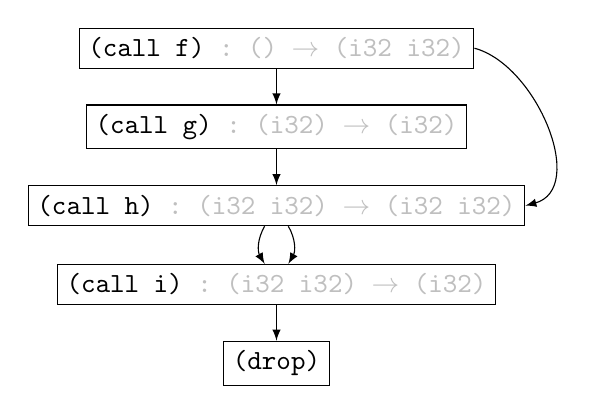
\begin{tikzpicture}
    \node[draw] (f) at (0, 0) {\texttt{(call f)\color{lightgray}~:~() $\to$ (i32 i32)}};
    \node[draw] (g) at (0, -1) {\texttt{(call g)\color{lightgray}~:~(i32) $\to$ (i32)}};
    \node[draw] (h) at (0, -2) {\texttt{(call h)\color{lightgray}~:~(i32 i32) $\to$ (i32 i32)}};
    \node[draw] (i) at (0, -3) {\texttt{(call i)\color{lightgray}~:~(i32 i32) $\to$ (i32)}};
    \node[draw] (d) at (0, -4) {\texttt{(drop)}};

    \draw[->,>=latex] (f) to (g);
    \draw[->,>=latex] (f.east) to[in=15, out=-15] (h.east);
    \draw[->,>=latex] (g) to (h);
    \draw[->,>=latex] (h) to[bend right] (i);
    \draw[->,>=latex] (h) to[bend left] (i);
    \draw[->,>=latex] (i) to (d);
  \end{tikzpicture}
  \caption{Non classical data flow with multiple return values.}\label{data-flow}
\end{figure}

\textsf{Watib}'s IR is closer to modern Wasm by representing the instructions in
a linear way. It allows to output code that use block parameters without
additional burden. We hope that this choice will enable different optimisations
and a better treatment of code written using WebAssembly's new features.

\section{Validation}\label{val}
Section~\ref{type} gives an overview of WebAssembly's type system, and
Section~\ref{algo} describes our implementation of a type checker for it. They
focus on the subtyping relation and the typing of instructions as the rest of
the validation is straightforward (checking that some names don't appear twice,
or that global variables' initial values are constant, etc.).
\subsection{WebAssembly's type system}\label{type}
We present the types used in WebAssembly and some declarative rules for
subtyping and typing of instructions. For more details, Section~2 of the
specification presents the abstract syntax of types, and Section~3 presents the
rules of typing and subtyping.
\subsubsection{Contexts}
We state all the following rules in an implicit \emph{context}, which we note
$C$ in the formal rules. Contexts are records; the only relevant field in the
following is \textsf{types} which maps type indices to \emph{defined types},
defined in~\ref{deft}.

\subsubsection{Value Types}
Wasm's main types are \emph{value types}, which we will note $t, t_1, t_2$, etc.
They are the types of values on the stack. They can be \emph{numeric types}
(\textsf{i32}, \textsf{f64}, etc.), \emph{vector types} (\textsf{v128}) or
\emph{reference types}. The latter category represents pointers to functions,
pointers to objects allocated on the heap (structures or arrays, called
\emph{aggregates}) or unboxed integers (using tagged pointers). Each reference
type is either nullable ($\refnullt ht$) or not ($\reft ht$), where $ht$ is a
\emph{heap type}. Such a type is either an \emph{abstract heap type} which we do
not detail here or a type index referring to one of the three following
possibilities.
\begin{itemize}\setlength{\itemsep}{0pt}
  \item \emph{Function types} are written
$\funt{t_1}^*\to{t_2}^*$ (recall that a function can have multiple outputs).
  \item \emph{Array types} are written $\arrt mut\ t$, where $mut$ denotes the
    mutability of the array. A mutability is \textsf{var} for a mutable array
    and \textsf{const} otherwise.
\item \emph{Structure types} are written $\strt {(mut\ t)}^*$.
\end{itemize}

\subsubsection{Instruction types}
The specification states inference rules to give \emph{instruction types} to
instructions. These types indicate which values on the stack an instruction
pops, which values it pushes and which local variables it sets\footnote{to
forbid, at the type level, using a variable not initialised yet}. We omit this
last piece of information in our presentation to stay simple. We write
instruction types like function types: ${t_1}^*\twoheadrightarrow{t_2}^*$ for an
instruction that pops ${t_1}^*$ and pushes ${t_2}^*$\footnote{the WebAssembly
standard uses the same arrow for instruction and function types, we distinguish
them for improved readability}. They obey the classical rule of subtyping for
functions as presented in~\cite{cardelli1988semantics}. An instruction can
accept smaller types as inputs and produce bigger types as outputs.
%% réécrire la suite ?
An additional subtyping rule reflects the stack-based semantics of Wasm: an
instruction can add arbitrary value types before the input and output types as
long as it adds the same on both. Figure~\ref{subinstr} presents a formal
version of these rules.

A sequence of instructions can then be typed by the composition of types derived
for each of its instruction. For instance, the sequence \texttt{(i32.const~0)
  (i32.const~0) i32.add} can be typed
$()\twoheadrightarrow(\text{\textsf{i32}})$, by giving the type
$(\text{\textsf{i32}})\twoheadrightarrow(\text{\textsf{i32}}\ \text{\textsf{i32}})$
to the second \textsf{i32.const} showing the need for the second subtyping rule.

\begin{figure}[h]
  \begin{mathpar}
    \inferrule{{\left(C\vdash t_1\leq t_1\right)}^*\\
      {\left(C\vdash t_2\leq t_2\right)}^*}
              {C\vdash {t_1}^*\twoheadrightarrow{t_2}^* \leq {t'_1}^*\twoheadrightarrow{t'_2}^*}\hspace{1in}
    \inferrule{\\}{C\vdash {t_1}^*\twoheadrightarrow{t_2}^* \leq t^*{t_1}^*\twoheadrightarrow t^*{t_2}^*}
  \end{mathpar}
  \caption{Subtyping rules for instruction types.}\label{subinstr}
\end{figure}

\subsubsection{Function and aggregate types}\label{func-aggr}
We now give details on the definitions and subtyping of function types and
aggregate types. As shown in Figure~\ref{tdef}, Wasm allows the definition of
mutually recursive types. Moreover, it supports \emph{declared and mutually
iso-recursive subtyping}.

\begin{figure}[h]
  \begin{lstlisting}
(rec
  (type $a (array (ref $b)))
  (type $b (struct (field (ref null $c))))
  (type $c (func (param (ref $a)) (result (ref $c)))))
  \end{lstlisting}
  \caption{Some type definitions.}\label{tdef}
\end{figure}

Function types are endowed with the same first rule described for instruction
types (the contravariant/covariant one). An array type $\arrt mut\ t$ is a
subtype of $\arrt mut'\ t'$ if $mut\ t\leq mut'\ t'$. It means that $mut$ is
equal to $mut'$ and that $t$ is a subtype of $t'$. When both types are mutable
we also require that $t'$ is a subtype of $t$, i.e.\ that both types are
equivalent. A structure type $\strt {(mut_i\ t_i)}_{i=1}^n {(mut\ t)}^*$ is a
subtype of $\strt {(mut'_i\ t'_i)}_{i=1}^n$, if $mut_i\ t_i\leq mut'_i\ t'_i$
for all $1\leq i\leq n$.

\subsubsection{Declared subtyping}
Wasm's subtyping is \emph{declared} as the subtyping relations between the types
defined have to be specified as part of the subtype's definition to be used.
Their validity can be checked with the type definition's validation. For
example, the definition of \texttt{\$pair} in Figure~\ref{ex} states that it is
a subtype of \texttt{\$pair-nil}. If the \texttt{sub \$pair-nil} part wasn't in
the definition, the type tests and the casts would be ill-typed, as a value can
be cast or tested against a type $rt$ if and only if $rt$ is a subtype of the
value's static type.

Each type definition can specify a supertype (the current specification only
allows one). A type can be a supertype if and only if it isn't \emph{final}.
Types declared in a program are final by default. The \texttt{sub} keyword in
the definition of \texttt{\$pair-nil} of Figure~\ref{ex} makes it non-final.

\subsubsection{Mutually iso-recursive subtyping}\label{deft}
We now give the intuition behind \emph{mutually iso-recursive subtyping};
see~\cite{rossberg2023mutually} for a full discussion. It is a way to support
subtyping in presence of mutually recursive type definitions, while avoiding
size blowups. When checking a block of such type definitions, we build an
internal representation where indices referring to types of the block have been
replaced by special indices of the form $\rect i$ where $i$ is the position of
the corresponding index in the block. A type is, then, a block of type
definitions and an index. For instance, the internal representation of the block
of Figure~\ref{tdef} is:
\begin{align*}
\rect\ (& (\arrt \cstt\reft \rect 1)\\
&(\strt\ (\cstt \refnullt \rect 2))\\
&(\funt\ (\reft \rect 0)\to (\reft \rect 2))).
\end{align*}
The \textsf{types} field of the context then maps each type index with a
reference to this block and an index (0 for \textsf{\$a}, 1 for \textsf{\$b},
etc.).

With this representation, a defined type $t$ will be a subtype of another
defined type $t'$ if they are equal or if the program declares $t$ as a subtype
of a subtype of $t'$.

\subsubsection{Unrolling}
Defined types only give a block of definitions and an index. To retrieve the
corresponding concrete type, one uses \emph{unrolling}. It consists of replacing
a defined type of the form $(\rect st^*).i$ by the $i^{\text{th}}$ type of $st$
where the indices of the form $\rect j$ have been replaced by $(\rect st^*).j$.

\subsection{A type checker for WebAssembly}\label{algo}
\subsubsection{The problem of transitivity}
The typing rules given by the third section of the specification are purely
declarative. They give more than one type to many instructions and rely on the
transitivity rule of subtyping, which can't be implemented as is. To check that
$t_1 \leq t_2$ in presence of transitivity, one can choose a third type to
compare it to $t_1$ and $t_2$, which complicates subtyping as $t_3$ is
arbitrary. We thus needed to adapt the rules to implement a type checker.

\subsubsection{Our solution}
\textsf{Watib}'s type checker is similar to the one shipped with the
specification. For the subtyping of \emph{value types}, we rewrote the rules to
have equivalent ones without the transitivity rules\footnote{they are
implemented by the function \texttt{<ht=} of the \texttt{Type/match.scm} and
reproduced in Appendix~\ref{subtyping}}, and for \emph{instruction types}, we
rely on a stack and most general types, as defined in~\ref{mgt}.

\subsubsection{Most general instruction types}\label{mgt}
Most instructions have a most general type (i.e.\ an admissible type for the
instruction that is a subtype of all its types) or do not return (like
unconditional branches). The typing rules for the latter are of the form
$i:{t_1}^*t^*\twoheadrightarrow {t_2}^*$ for all $t_1$ and $t_2$, but where
$t^*$ is fixed. We represent it as $t^*\twoheadrightarrow
(\text{\textsf{poly}})$, where \textsf{poly} is a special symbol indicating that
the stack can be whatever we need it to be. It can be thought as a type variable
on which we do not perform explicit unification. When we refer to the type one
of those instruction, we mean its most general type or the type with the
\textsf{poly} symbol, these types are contained in the file
\texttt{Val/instruction-types.sch}. The instructions that do not fall in either
category (for instance, \textsf{ref.as\_non\_null} has type $\refnullt ht\to
\reft ht$ for all heap type $ht$) are treated in a separate function, they peek
on the stack to compute their output type, avoiding the use of type variables.

\subsubsection{The algorithm}
To check a sequence of instructions we maintain an internal state recording the
types of the elements present on the stack and then check instruction in order,
instead of analysing each instruction individually and checking that the types
compose well.

We describe how one instruction $i$ modifies the state of this stack. Either we
treat the instruction in an ad-hoc way (function \texttt{adhoc-instr}), or we
apply the following procedure (function \texttt{valid-instr}) if the instruction
falls in one of the two categories of~\ref{mgt}:
\begin{itemize}\setlength{\itemsep}{0pt}
\item Let ${t_n\ldots t_1}^*\twoheadrightarrow{t'}^*$ be the type of $i$.
\item Check that the $j^{\text{th}}$ type on the stack is a subtype of $t_j$ and
  pop it, for $j$ from $1$ to $n$. If the stack is equal to \textsf{(poly)}, for
  all $j$, consider that the $j^{\text{th}}$ type on the stack is $\bot$, making
  the previous test successful.
\item If ${t'}^*$ is equal to \textsf{(poly)}, replace the stack by
  \textsf{(poly)}, otherwise push the return types on top of the stack.
\end{itemize}

\subsubsection{Type checking blocks}
To check a block against a given type, set the parameter types as initial state
of the stack and compare the final the state of the stack with the expected
type. For that final check, pop types from the stack and check that they
are subtype of the expected ones. End by checking that the resulting stack is
empty or equal to \textsf{(poly)}.

\section{Optimisation}\label{opt}
\textsf{Watib} performs several optimisation passes that all maintain type
information. Our optimiser is transformation-based: it applies sequentially
small indepedent code transformations. As noted in the introduction
of~\cite{jones1998transformation}, this design increases modularity of the the
toolchain, and it facilitates experimenting with the order of the passes.

%% As we show it later, some code is unnecessary execution-wise but
%% needs to be kept to maintain well-typedness.

\subsection{Generic optimisations}
We start by reviewing optimisations which benefit the others, by giving more
precise information or removing generated useless code. They are generic in the
sense that they are applied in most optimising
compilers~\cite{muchnick1997advanced}.

\subsubsection{Copy Propagation}
When a variable $x$ receives the value of another variable $y$, one can replace
references to $x$ with references to $y$ until the next assignment to $x$ or
$y$. The Copy Propagation pass performs such replacements. We took inspiration
from Muchnick's~\cite[Section~12.5]{muchnick1997advanced} approach to local copy
propagation for our implementation.

We traverse a sequence of instruction while maintaining a table \textsf{acp}
which indicates if a variable contains the value of another one, and we
associate each enclosing label to a list of such tables. We then apply the
following procedure when encountering an instruction $i$:
\begin{itemize}\setlength{\itemsep}{0pt}
  \item When $i$ assigns the value of a variable $y$ to another
    variable $x$, update \textsf{acp} with $x$ pointing to $y$. Replace each
    occurence of $x$ in \textsf{acp} by $y$. Otherwise, all the assignments
    concerning $x$ are removed from the table.
  \item When $i$ accesses a variable $x$ and that $\textsf{acp}[x]$,
    modify the instruction to access $\textsf{acp}[x]$.
  \item When $i$ can branch to a label $l$, append the current table to
    the list associated to $l$.
  \item When $i$ is a block of label $l$, associate an empty list to $l$. The
    table after the block corresponds to the upper-bound of all the tables
    associated to $l$ and $\textsf{acp}$ at the end of the block. The upper
    bound of a list of tables assigns $y$ to the $x$ if all tables do and gives
    no information on $x$ otherwise.
  \item When $i$ is a loop, reset \textsf{acp} to remove all the
    assignments as we may jump to the beginning of the loop from later in the
    block\footnote{this is suboptimal for global copy propagation, but it is
    sufficient for the code we get, and this optimisation could be replaced by
    the optimisation we describe in~\ref{sbbv}}. Then treat the loop's body.
  \item When $i$ is an if statement, treat each branch as a block and
    take the upper bound of the two resulting tables.
  \item When protecting a block with some \textsf{catch} clauses, append
    the table indicating no assignment to all the labels these clauses can jump
    to. Once again this is coarse.
\end{itemize}

At the end of each block, remove all the assignments in \textsf{acp} whose
right-hand side is uninitialised in the parent block.
\subsubsection{Pure Drops Elimination}
When an instruction produces a single value that is then popped by a
\textsf{drop}, both instructions are useless, except for the side effects of the
former. The Pure Drops Elimination pass removes such patterns that do no side
effects apart from popping values on the stack. When a removed instruction
popped values of the stack, each popped value gets a corresponding \textsf{drop}
that can be removed by the pass.

\subsubsection{Constant Folding}
The Constant Folding pass performs computations whose results at compile time.
For instance, if statements on a constant values can be replaced by the
corresponding branch.

\subsubsection{Unreachable Code Elimination}
The Unreachable Code Elimination pass eliminates some instructions that are
known to never execute (the ones after a \textsf{return} for instance). However,
some dead code is needed for validation. For instance, removing the
\textsf{unreachable} instruction at the end of the function of Figure~\ref{ex}
makes it ill-typed, even though both branches of the if statement return. The
\textsf{if} instruction puts nothing on the stack while the function expects an
\textsf{i32} on top of the stack as it is its declared return type. An
\textsf{unreachable} instruction replaces the unreachable code when it isn't
preceded by an instruction of polymorphic return type. The unreachable code can
be deleted otherwise.

\subsubsection{Peephole Optimisation}
Some small patterns in Wasm code is equivalent to code that is smaller or
faster. For instance a sequence of \textsf{local.set} and \textsf{local.get}
with the same variable is equivalent to a \textsf{local.tee} which assigns to a
variable the value on top of the stack without popping it. The Peephole
Optimisation pass recognises such patterns and replaces them.

%% \subsubsection{Type propagation}
%% This one is not an optimisation \emph{per se}. It only refines type annotations
%% of variables in the IR. When a variable is assigned a value, the type of this
%% value (which may be a strict subtype of the variable's declared type) is set as
%% the actual output type of each variable access, until it is modified.

\subsection{Wasm specific optimisations}
We now review more Wasm-specific optimisations and detail in which way they use
the previous ones.
\subsubsection{Cast Elimination}
The Cast Elimination pass removes redundant casts and replaces type tests by
constants if their result can be determined. Such casts and tests could be
introduced by copy-propagation as when we may replace a variable with another
one of a smaller type or by the next optimisation. To stay conservative about
side effects, eliminated tests are replaced by a \textsf{drop} and the result of
the test, which is a constant. Pure Drop Elimination will remove some useless
computation. Constant folding will propagate the result of the test.

To check for type tests to eliminate, we compare the argument's actual type
(which may be smaller than its static type) against the type it is tested for.
For casts, we only check against the static type as the cast can be necessary to
maintain well-typedness.

\subsubsection{Type-Dependent Control Flow Rewriting}
A common pattern in the Wasm code generated during the compilation of
dynamically typed programming languages, such as Bigloo, is a branching on a
type test followed by the use of casts in the branch where the test is
successful, like in Figure~\ref{ex}. If Wasm wasn't statically typed, these
casts could be removed by an optimising compiler that would determine that they
are redundant.

The instruction $\broncast l\ rt_1\ rt_2$, where $l$ is a label expecting a
value of type $rt_2$ as parameter and $rt_1\geq rt_2$ are reference types, can
avoid useless type tests, by combining branching and casting. While
\textsf{ref.cast} traps when the type test fails, \textsf{br\_on\_cast} allows
arbitrary (structured) jumps. A call to this instruction with a value of type
$rt_1$ on top of the stack applies the following procedure:
\begin{itemize}\setlength{\itemsep}{0pt}
  \item Check this value against the type $rt_2$.
  \item If the type test succeeded, branch to label $l$ with the value on top of
    the stack as a parameter.
  \item Else, continue the execution without modifying the stack.
\end{itemize}
\begin{figure}[h!]
  \centering
  \begin{tabular}{c c c}
    \begin{minipage}{\widthof{\texttt{(if (ref.test (ref \$pair)}}}
\begin{verbatim}
(if (ref.test (ref $pair)
      (local.get $x))
  (then B1)
  (else B2))
\end{verbatim}
\end{minipage}
    &
    $\rightarrow$
    &
\begin{minipage}{\widthof{\texttt{....(br\_on\_cast \$then (ref \$pair-nil)}}}
\begin{verbatim}
(local $y (ref $pair))
(block $end
  (block $then (result (ref $pair))
    (br_on_cast $then (ref $pair-nil)
                      (ref $pair)
      (local.get $l))
    (drop)
    B2
    (br $end))
  (local.set $y)
  B1[$x:=$y])
\end{verbatim}
\end{minipage}
  \end{tabular}
  \caption{General form of type-dependent control flow rewriting.}\label{br}
\end{figure}


This pass replaces \textsf{if} instructions which branch on a $(\reftest
rt\ (\localget x))$ by calls to \textsf{br\_on\_cast}, as Figure~\ref{br} shows
it. It adds a local variable $y$ of type $rt$ and creates a new block labelled
$l$ with a parameter of type $rt$. The else branch follows the
\textsf{br\_on\_cast} which branches to $l$. The block labeled by $l$ puts its
parameter in the local variable $y$ and replaces $x$ by $y$ in the then branch
following the same procedure as Copy Propagation. This whole code is contained
in a block which the else branch goes to at the end. Cast Elimination can then
removes useless tests.

While the code after the transformation is bigger, some instructions \texttt{(br
  \$end)} can be removed on real examples.

\section{Benchmarks}\label{bench}
\subsubsection{The methodology}
We tested our toolchain by running, on Bigloo's Wasm backend, a subset of the
R7RS benchmarks~\cite{r7rsbench}, the standard benchmark suite for Scheme. We
compare the execution time using \textsf{watib} with all of its optimisation
passes enabled with the previous backend using \textsf{wasm-as} with no
optimisation enabled.
\begin{figure}[h!]
  %\centering
  \includegraphics[width=1\textwidth]{report/bench.pdf}
  \caption{Benchmarks against the a subset of the R7RS benchmarks suite.}\label{r7rs}
\end{figure}
\subsubsection{The results}
Figure~\ref{r7rs} shows the results of our benchmarks. The red line indicates
the performance when all \textsf{watib} are enabled, and the blue bars indicates
the performance without any of them. Our optimisation passes do not impact
running time of most benchmarks. There is a noticeable negative impact on only
\texttt{conform} which runs 10\% slower with optimisations. Two benchmarks
benefit from the optimisations: \texttt{early} and \texttt{fib} with a
respective speedup of 17\% and 10\%.

We are investigating the reasons of the slowdown on \texttt{conform}; we found
that:
\begin{itemize}
  \item Disabling the Cast Elimination pass solves the issue.
  \item The SpiderMonkey engine doesn't suffer from the same performance
    penalty.
  \item V8's TurboFan, a multi-pass compiler, doesn't suffer either from the
    same performance penalty.
\end{itemize}
\section{Static Basic Block Versioning}\label{sbbv}
We present here a new pass we are working on. \textsf{Watib} does not support
this pass yet, but we implemented the necessary machinery to experiment with
hand-optimised programs.
\subsubsection{Control-Flow Graphs}\label{cfg}
Some optimisations and code transformations manipulate a \emph{Control-Flow
Graph} (CFG). It is a graph whose nodes are \emph{basic blocks} (sequences of
instructions that do not affect the control flow, here Wasm instructions) and
arcs represent potential jumps. To reflect the typing discipline of Wasm, we
consider CFGs whose basic blocks have instruction types.

\subsubsection{The optimisation}
We are working to adapt Static Basic Block Versioning or
SBBV~\cite{melanccon2024static} (which works on CFGs) to WebAssembly. This
optimisation produces different versions of a same basic block. Each version has
more precise information about the context it begins in (with information on
local variables for instance) and can specialise its instructions to reflect
that. In \textsf{watib}, SSBV could subsume Copy Propagation and Cast
Elimination.

\subsubsection{Construction of a control-flow graph}
Constructing a CFG from a Wasm program is straightforward except for exceptions
which we don't support yet. One only needs to follow the program's control flow,
while keeping a state of the types on the stack to annotate the basic blocks
with types.

\subsubsection{Reconstruction of Wasm}
As we don't have a general goto instruction, the translation of a CFG to a a
valid Wasm program isn't as easy. To reconstruct structured control flow, we
implement the algorithm described in~\cite{ramsey2022beyond}. This algorithm
relies on the \emph{dominance tree} of the CFG, which we compute using the
algorithm of~\cite{cooper2001simple}. We adaptated Ramsey's algorithm to support
\textsf{br\_on\_cast} as a way to jump out of a block and to use the type
annotations on the CFG to type the Wasm blocks. The latter addition allows
preserving block parameters and output values in the input program.

\subsubsection{Reducibility}
Ramsey's algorithm works on \emph{reducible} CFGs. Intuitively, a CFG is
reducible when each loop has a single entry point. WebAssembly's structured
control flow only produce such CFGs. But the SBBV we work on can modify the CFG
of a program with no guaranty on reducibility, at least in its current
formulation.

\subsubsection{Fixing non-reducibility}
We are considering two different ways to obtain a reducible CFG after this pass.

On the one hand, the GHC compiler, which uses Ramsey's algorithm, makes CFGs
reducible through \emph{node-splitting}. This technique duplicates problematic
nodes such that each copy has a unique incoming arc, until the resulting graph
is reducible. With this method, the reducible graph obtained executes exactly
the same instructions as the original one, at the cost of a size expansion,
which can be exponential~\cite{carter2003folklore}. GHC implements node
splitting~\cite[Appendix~A]{ramsey2022beyond} with a greedy algorithm. A more
elaborate method obtains better results~\cite{janssen1997making}.

On the other hand, non-reducibility appears when SBBV duplicates the head of a
loop and that there are arcs between the different versions of the same loop. We
can then make the graph reducible by creating a new node that serve as a common
head for all the versions of the loop. Instead of jumping to a head, a node
would branch to this new head indicating which version of the loop it targets.
The new head would then branch to one of the previous heads with a
\textsf{br\_table}. This approach solves size explosion problem but adds
execution overhead.

We also plan to test not applying the optimisation to some parts of the graph
where it generates a non-reducible CFG.

\section{Conclusion}
We reviewed and motivated some of \textsf{watib}'s design choices and we
compared it to existing toolchains. We also detailed the type checking
algorithm, and the optimisation passes.


\renewcommand{\baselinestretch}{1}
\printbibliography
\renewcommand{\baselinestretch}{1.05}

\newpage
\appendix
\section{Wasm-as' extensions to the specification}\label{wasmasex}
We try to list wasm-as' extensions to the spec, i.e.\ code modification made by
wasm-as silently that do not appear specification. To our knowledge, this
behaviours are not documented. The list is non-exhaustive. Feel free to contact
us if you find anything missing.
\subsection{\textsf{Unreachable} insertion}
Wasm-as tend to replace dead code code by \textsf{unreachable} and add
\textsf{unreachable} after blocks that don't exit. While semantically
preserving, this transformation can transform invalid code in valid code. For
instance, the following function is not well-typed according to the spec. But
wasm-as inserts an \textsf{unreachable} at the end, making it well-typed.
\begin{lstlisting}
(func (result i32)
  (if (i32.const 0)
    (then (return (i32.const 0)))
    (else (return (i32.const 0)))))
\end{lstlisting}

In the following piece of code, the \textsf{br} is not well-typed but wasm-as accepts
it:
\begin{lstlisting}
(func
  (result i32)
  (block $main (result i32)
    (i32.const 0)
    (if
      (then (return (i32.const 0)))
      (else (return (i32.const 0))))
    (br $main)))
\end{lstlisting}
\subsection{Automatic function reference declaration}
According to the specification, functions appearing in a \textsf{ref.func} have to
appear outside the function bodies (in a global or in an elem section). Wasm-as
puts all the undeclared function reference in an \textsf{elem declare func} section.

\subsection{Sign extension insertion for packed get}
According to the specification, when using \textsf{array.get} or
\textsf{struct.get} on a packed field (\textsf{i8} or \textsf{i16}), a sign
extension has to be specified. It means that either \textsf{.get\_u} or
\textsf{.get\_s} has to be used. Wasm-as allows \textsf{.get} instructions on
packed types, defaulting to unsigned.

\subsection{Replacement of block input values by locals}
Binaryen's README mentions that block input values are represented in the IR by
\textsf{pop} subexpressions for \textsf{catch} blocks and not supported for the
others. It is not mentioned that code using block input values will be replaced
by the use local variables. For instance, the following code:
\begin{lstlisting}
(i32.const 0)
(block (param i32)
  (drop))
\end{lstlisting}
is assembled to:
\begin{lstlisting}
(i32.const 0)
(local.set 0)
(local.get 0)
(drop)
\end{lstlisting}
\section{Matching rules for heap types}\label{subtyping}
\begin{mathpar}
  \inferrule{t_1 = t_2}{C\vdash t_1\leq t_2}\hfill
  \inferrule{\\}{C\vdash \bot\leq t}\hfill
  \inferrule{C\vdash C.\text{\textsf{types}}[x]\leq t}{C\vdash x \leq t}\hfill
  \inferrule{C\vdash t \leq C.\text{\textsf{types}}[x]}{C\vdash t \leq x}\\
  \inferrule{C\vdash t\leq\text{\textsf{any}}}
            {C\vdash\text{\textsf{none}}\leq t}\hfill
  \inferrule{C\vdash t\leq\text{\textsf{func}}}
            {C\vdash\text{\textsf{nofunc}}\leq t}\hfill
  \inferrule{C\vdash t\leq\text{\textsf{extern}}}
            {C\vdash\text{\textsf{noextern}}\leq t}\hfill
  \inferrule{C\vdash t\leq\text{\textsf{exn}}}
            {C\vdash\text{\textsf{noexn}}\leq t}\\
  \inferrule{C\vdash t\leq\text{\textsf{any}}}
            {C\vdash t\leq\text{\textsf{eq}}}\hfill
  \inferrule{\\}{C\vdash\text{\textsf{i31}}\leq\text{\textsf{eq}}}\hfill
  \inferrule{\\}{C\vdash\text{\textsf{struct}}\leq\text{\textsf{eq}}}\hfill
  \inferrule{\\}{C\vdash\text{\textsf{array}}\leq\text{\textsf{eq}}}\\
  \inferrule{\text{\textsf{unroll}} (deftype)= (symbol\ldots)}
            {C\vdash deftype\leq symbol}\hfill
\inferrule{\text{\textsf{unroll}} (deftype)= (symbol\ldots)\\ C\vdash symbol\leq\text{\textsf{eq}}}
            {C\vdash deftype\leq\text{\textsf{eq}}}
\end{mathpar}
\end{document}
